\chapter{Introduction}


\section{Motivation/Problem}
There is a number of reasons to expect an extending demand for higher network throughput capabilities for mobile devices. This demand is even more urging when looking at applications working with video streaming. The following two sections look at two driving forces behind this trend.

\subsection{Trends in mobile internet usage}
The transmission of video information in realtime requires a higher throughput capability than the transmission of voice or still picture information does. Because of this fact, the growing usage of mobile video results in much greater challenges than the increased usage of other services.
With mobile video being up to 50\% of mobile internet traffic, as the Cisco visual networking index suggests, we need to increase the available throughput as much as possible.
\subsection{Trends in mobile device development}
The capabilities of mobile devices keep improving. On one hand the devices are capable of using new network infrastructure like LTE-Networks, which allows them to communicate at a faster rate. On the other hand, their ability to process multimedia content is improving. One of the often advertised characteristics of mobile devices is the resolution of their display. At this point devices with a resolution of 1920x1080 Pixels are available. However the manufacturers are already promising to bring devices with a resolution of 4096x2160 Pixels. If users try to download video content at the apropriate resolution to make full use of their device over the mobile networks, they will use up a lot more of the network capabilities than they currently do. 
\subsection{Mobile network operators}
One obvious solution to this problem is the "dumb fat pipe" approach. However this is a solution only the mobile network providers can implement and it requires investment on their side, which might result in increased fees for the customer. Even if the network operator provides almost ideal coverage, a number of problems might appear when communicating over a wireless link. The changing distance to the base station and external interference as well as multi-path propagation might result in signal coverage fluctuation.
Additionaly, a number of mobile network providers in Germany are currently offering monthly plans with an unlimited amount of data, which can be transmitted with the limitation of an artificialy decreased transmission speed after a certain amount of data received. For a user of such a network plan it might be tempting to circumvent the limited throughput through cooperation with other users in the same situation.

In the following we try to evaluate the concept of collaborative video streaming and its implementation, based on ColStream, the system introduced in \cite{ColStream}.
%additional reason. you are not currently qualified to use the available network (wrong frequancy) sharing helps.

%traveling by bus example

\section{Overview of ColStream}
The following sections introduce ColStream as a possible solution to the previously described problems. They show the scenario it is assumed to be used in and how it intends to solve the problem of limited throughput over a 4G/LTE connection.
% \subsection{Historical Information}
The name ColStream is a contraction of the words collaborative and streaming. It was introduced in 2014 by Mingyang Zhong, Peizhao Hu, Jadwiga Indulska and Mohan J Kurnar as an approach to inprove the video streaming capabilities of one mobile device through cooperation with other devices. Its concept was implemented as an Android application.
\subsection{Scenario}
\begin{figure}[hbtp]
\centering
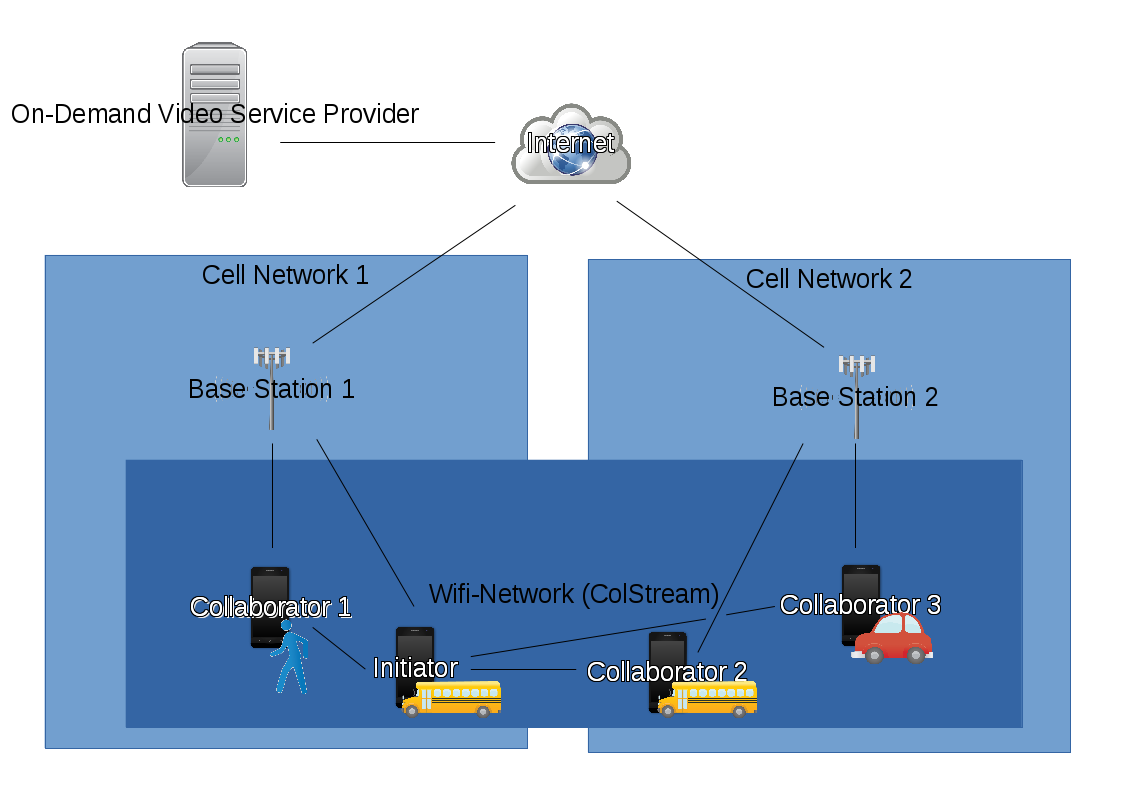
\includegraphics[scale=.6]{figures/Overview.png}
\caption{Overview of the idea of ColStream}
\label{ColStreamIdea}
\end{figure}
In \cite{ColStream} Zhong et al. describe a scenario of a person accessing a high-definition video stream through a mobile device over a 4G/LTE network. Figure \ref{ColStreamIdea} illustrates this scenario. The mobile network might experience interference or not be available at all times. To compensate for these limitations the mobile device connects over Wi-Fi to other mobile devices and negotiates with them the transmission of parts of the video stream over their 4G/LTE connection. As the location of the person is changing so is the level of experienced interference and the number and capabilities of devices surrounding it. ColStream promises to adopt to these changes and through negotiations to find the best available combilation of collaboration partners. The base for this negotiation process is provided by a virtual currency through which the video consuming participant can pay others who offer him their bandwidth.



\section{Related Work}\label{relWork}
There are a number of concepts and implementations that try to leverage cooperation to improve user experience when streaming or downloading information.
\subsection{Collaborative Download}
There are several Peer to Peer (P2P) networks that allow collaborative download. One famous example is the BitTorrent network which can be used to distribute large files like Operating System images with limited server capacity. Even though a streaming system with questionable legality was created based on it, these systems were designed to maximize the availability of a download, not its speed \cite{P2P}. When looking at streaming video to mobile devices, we assume the 3G/LTE connection to be the bottleneck. In this situation, the usage of such a P2P-system over this connection is of no advantage to us. While we could try to share information with our peers over Wi-Fi, we can not assume to have enough peers interested in the same information in range of our Wi-Fi connection.  
\subsubsection{CStream}
CStream \cite{CStream} appears to be a system very similar to ColStream, even in its naming, in which the C is short for collaborative. Both focus on the improvement of video streaming performance. However CStream does not focus on the mobile scenario. Instead it intends to apply this approach to a wider range of scenarios specifically including the combination of several wired connections.
\subsubsection{COMBINE}
COMBINE \cite{COMBINE} is a system designed to improve the download speed of files by using the 3G/LTE connection of other mobile devices, which can be reached over Wi-Fi. So it is very similar to CosStream, however it was designed without the realtime demands that appear when handling a video stream. Additionaly its current implementation only works on notebooks and PCs, not on smartphones or tablets. These two classes of devices still differ in many ways based on their processing power, the time they can work without recharging, the probability to find one of those devices turned on in your Wi-Fi range. We consider this to be problematic when evaluating the behaviour of this system on what we consider to be mobile devices.
\subsection{Incentive Systems}
One of the most important parts of ColStream is its incentive system, which is necessary to motivate users to offer their unused throughput to others. Unfortunately while the negotiation process for payment is discussed in depth, it is unclear if the system has any means to motivate the user to look for pazments to earn and to offer his available throughput to do so.In the following section we list a number of systems with a simmilar problem and their incentive approach.
\subsubsection{BitTorrent}
P2P networks face a similar problem. BitTorrent tries to evaluate the effort a user is providing based on his ratio of up- and downloads in relation to the resources available to him, specifically storage space and network access. Users can be punished for having a low ratio of uploads to downloads by restricting the download speed\cite{cohen2003incentives}.
\subsubsection{Webservices}
A number of webservices like reddit.com or duolingo.com allow the user to earn virtual points similar to the payments a user receives in ColStream. In the extreme case of reddit these points have no use besides showing others that a user has made valuable contributions. 


%%\label{chap:SomeStuff}

%% Note that the citations in this chapter use the journal and 
%% arXiv keys: I used the SLAC-SPIRES online BibTeX retriever 
%% to build my bibliography. There are also quite a few non-standard
%% macros, which come from my personal collection. You can have them
%% if you want, or I might get round to properly releasing them at 
%% some point myself.

%%\chapterquote{Laws were made to be broken.}%
%%{Christopher North, 1785--1854}%: Blackwood's Magazine May 1830

%%Symmetries, either intact or broken, have proved to be at the heart
%%of how matter interacts. The Standard Model of fundamental interactions
%%(SM) is composed of three independent continuous symmetry groups denoted 
%%$\SUgroup{3} \times \SUgroup{2} \times \Ugroup{1}$, representing the 
%%strong force, weak isospin and hypercharge 
%%respectively~\cite{Phys.Rev.Lett.19.1264, Phys.Rev.D2.1285,hep-ph/0410370}.

%%\section{Neutral meson mixing}
%%\label{sec:neutralmixing}
%%We can go a long way with an effective Hamiltonian approach in
%%canonical single-particle quantum mechanics. To do this we construct
%%a wavefunction from a combination of a generic neutral meson state 
%%$\ket{\Xzero}$ and its anti-state $\ket{\Xzerobar}$:
%%%
%%\begin{equation}
%%  \ket{\psi(t)} = a(t)\ket{\Xzero} + b(t)\ket{\Xzerobar}
%%\end{equation}
%
%%which is governed by a time-dependent matrix differential equation,
%
%%\begin{equation}
%%  \I \pdByd{}{t} \colvector{a \\ b}
%%  =  
%%  \underbrace{%
%%  \twomatrix{ M_{11}-\frac{\I}{2}\Gamma_{11}           
%%            & M_{12}-\frac{\I}{2}\Gamma_{12} }
%%            { M_{12}^\ast-\frac{\I}{2}\Gamma_{12}^\ast 
%%            & M_{22}-\frac{\I}{2}\Gamma_{22} }
%%  }_{\boldmatrix{H}}
%%  \colvector{a \\ b}
%%  .
%%\end{equation}